Our climate is changing and the associated impacts are being felt from the 
global level down to our local community. Increasing temperatures, rising sea 
level, and changing precipitation patterns are leading to cascading and 
interconnected impacts on our health, our environment, and our economic 
vitality. We are experiencing these climate hazards as flooding, heat waves, 
and drought. Understanding how these changes are affecting our community will 
help us address their impacts by increasing our resilience through smarter 
decision-making, land-use planning, and adaptation. Natural resources are an 
important asset in planning for resilience, managing climate risks, and 
recovering from extreme weather events ~\citep{haeckel2014}. A brief overview of 
the effects of our changing climate follows; additional background information 
is found in the appendix section.
\par
We are seeing \textbf{temperature} increases that are making our summers hotter 
and our winters warmer and shorter; annual average temperatures have increased 
\textcolor{red}{2}$\si{\degree}$F and winter temperatures have increased 
\textcolor{red}{5}$\si{\degree}$F in New York since 1970. Temperature fluctuations 
are impacting the growing season of our food crops and the beauty of our 
autumnal leaf season. These changes, in turn, are impacting our produce and 
tourism economies.
\par
The incidence of extreme temperatures is also increasing. ``By mid-century, 
the Hudson Valley could annually experience 3-12 days above 
\textcolor{red}{95}$\si{\degree}$F, and four to seven heat waves that last 1-2 days 
longer than average'' ~\citep{Zemaitis2018}. ``Climate Impacts on Human Health'' 
notes that these increases will put in danger the lives of our vulnerable 
residents—our children and elders—from extreme heat and poor air quality. The 
\textit{National Climate Assessment} further notes that increasing temperatures 
are projected to result in decreased air quality from increase ground-level 
ozone and/or particulate matter air pollution. ``Ground-level ozone (a key 
component of smog) is associated with many health problems, such as diminished 
lung function, increased hospital admissions and emergency room visits for 
asthma, and increases in premature deaths'' ~\citep{melillo2014}. 
Ground-level ozone and particulate air matter will be of special concern in 
Orange County because cars are the greatest source of air pollution, given the 
high single-occupancy vehicle rate and commuting distances in Orange County; 
traffic on Stewart Airport, I-84 and I-87, and nearby power plants will also 
play a role. (Orange County is fortunate to have seen a general improvement in 
air quality since 1999 across many ~\gls{naaqs} metrics, resulting in a decreased 
number of unhealthy days for people suffering from asthma, lung disease, and 
heart disease as well as for older adults, children, people engaged in outdoor 
activities, and the general population ~\citep{aircompare, ocnysenvironmental}. 
\par
Our precipitation patterns are also changing. The Northeast and New York have 
seen a 71\% increase in heavy precipitation events between 1958 and 2012, that 
have resulted in more frequent and costly flooding \citep{melillo2014}. 
While the reduction in forested and undeveloped land cover plays a role in 
increased flooding, even these pervious areas cannot absorb the intense rainfall 
from heavy precipitation events, becoming water-logged and reducing the amount 
of water that reaches our aquifers. Our aquifers are also seeing a lower 
recharge rate due to the reduction in snowpack, caused by increased winter 
temperature. Snowpack decline is also negatively impacting our winter 
recreational industries and economy.
\par
Rising sea levels are affecting all waterfront communities, including Hudson 
River estuary communities. ``Since 1900, sea level in the lower Hudson has 
risen one foot'' ~\citep{haeckel2014}, with an additional projected rise of up 
to 75 inch, or over six feet, for the Lower Hudson Valley by the end of this 
century ~\citep{horton2014climate}. Rising sea levels will lead to flooding along 
estuary shorelines and tidal tributary waters, particularly in low lying areas. 
Flooding will be compounded by heavy storm surges, such as those we experienced 
from Hurricanes Irene and Sandy, and intense rainfall leading to additional 
tributary and stormwater flooding.

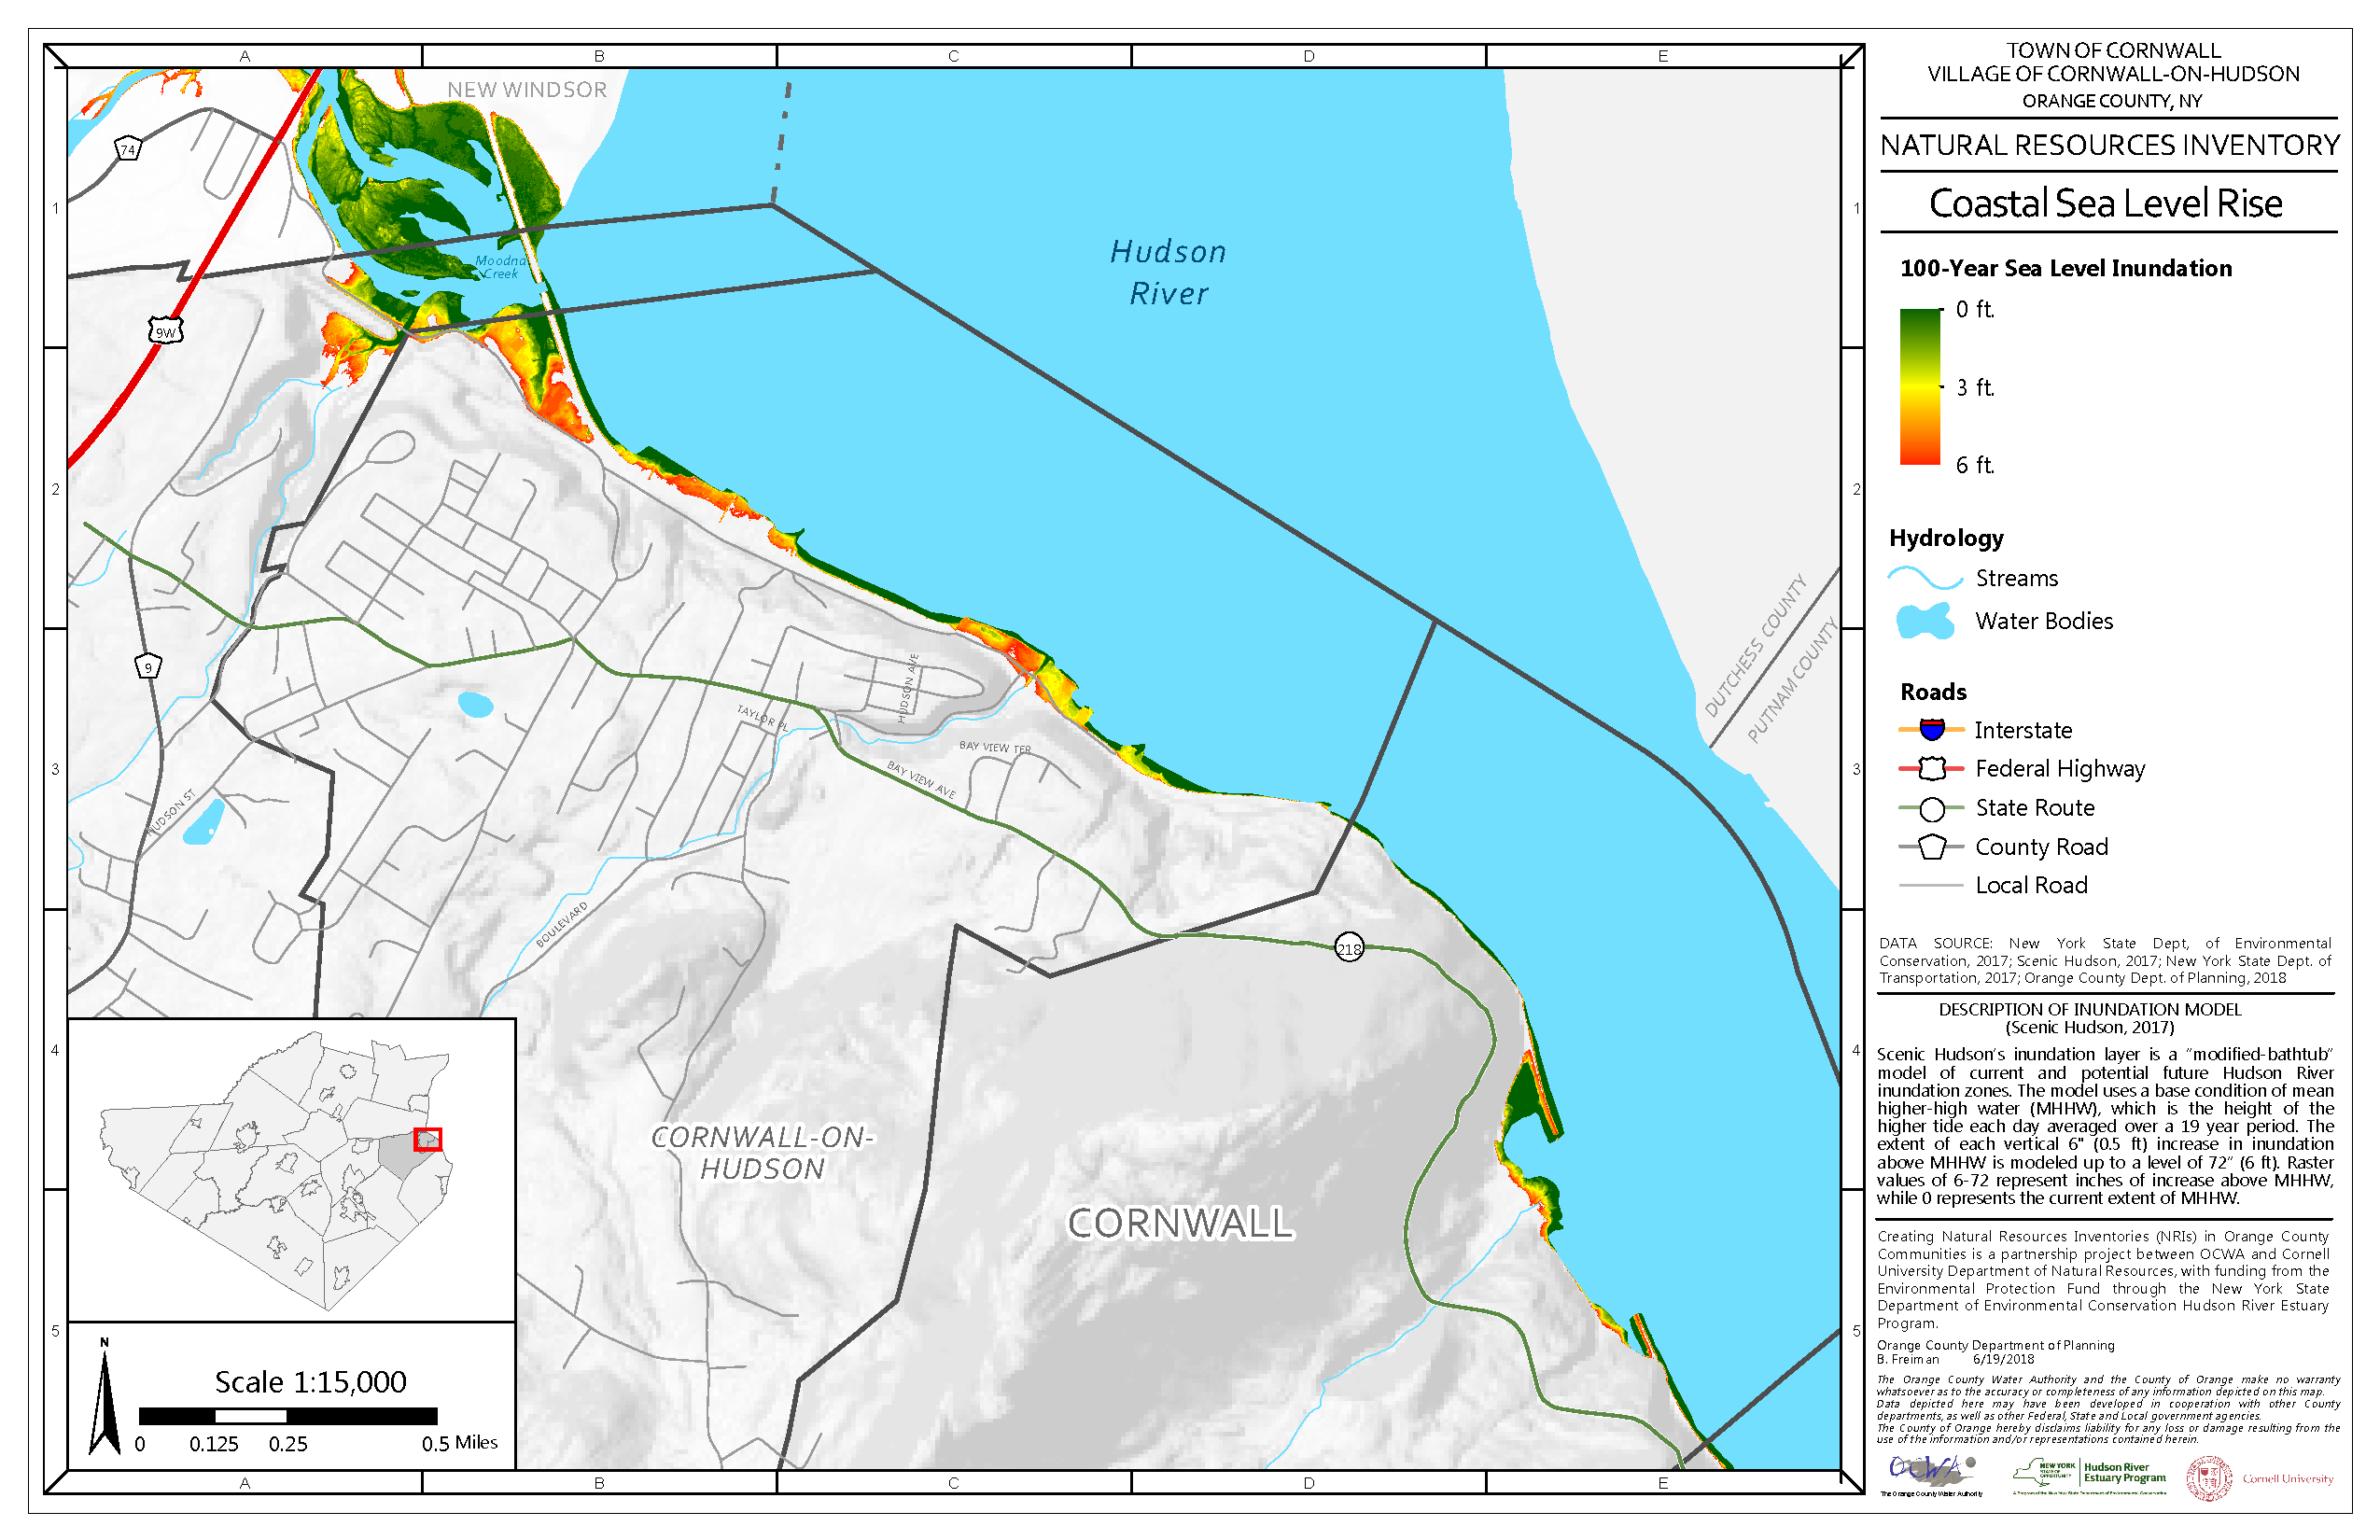
\includepdf[pages=-,fitpaper]{cornwall_maps/CoastalClimateChange.pdf}\label{map:coastalclimatechange}
\subsection*{Coastal Sea Level Rise Map}
The Village of Cornwall-on-Hudson has significant shoreline on the Hudson River 
and is vulnerable to sea level rise. This image shows two important community 
assets: Donahue Memorial Park in the Village and the wastewater treatment plant 
in the Town at the mouth of the Moodna (source: New York Climate Change Science 
Clearinghouse).
\par
The Coastal Sea Level Rise map depicts the areas of future inundation that 
Village and Cornwall residents would experience from a rising Hudson River. In 
a 3-foot sea level rise, 100-year flood scenario (yellow on the map), key 
portions of the wastewater treatment plant are submerged and Shore Road is 
almost inaccessible; we lose roughly half of Donahue Memorial Park to the 
Hudson. In a 6-foot sea level rise scenario (in red), the entire wastewater 
treatment site is in the Hudson and Donahue Memorial Park ceases to exist. Our 
access to the river becomes the train tracks.
\par
In addition to the riverfront inundation modeled in the map, this image shows 
the resulting flooding that would reach inland (orange) as a result of a 6-foot 
sea level rise. 

\subsection*{Becoming a Climate-Resilient 
Cornwall}\label{subsec:climateresilient}
We are already seeing the costly effects of our changing climate and have 
responded to these impacts in different ways. For example, we have protected 
sewage treatment facilities by raising their height, repaired drainage 
destroyed by heavy storms, cleared away left-over storm debris, and cleaned up 
our flooded houses. Understanding the best-case and worst-case scenario 
projections, however, have armed us with the ability to take proactive measures 
to make our community more resilient to the impacts of climate-caused hazards. 
\par
Below is a short list of actions that the New York State Climate Smart 
Communities Program recommends that communities like ours pursue as part of any 
resiliency planning and as a means of responding to the expected federal and 
state mandates for ``strong coastal and floodplain construction standards and 
pre-disaster mitigation planning.''
\begin{enumerate}
    \item Conduct an assessment of municipal and county documents, where 
applicable, to determine the degree to which plans, ordinances, and strategies 
incorporate resiliency planning.
    \item Develop or update a vulnerability assessment to identify ``vulnerable 
    populations, businesses, infrastructure, and natural resources.'' The 
    assessment process assists municipalities with building their knowledge and 
    ability to plan for climate-caused hazards.
    \item Engage the public in identifying the effects of historic storms 
    and make available to the public ``information on the natural and 
    beneficial 
    functions of floodplains, wetlands, and green infrastructure.'' 
    Periodically conduct storm preparedness outreach to residents and 
    businesses.
    \item Develop or update a heat emergency plan. Explore the expansion of 
    cooling centers.
    \item Increase shading in public spaces with trees and other structures.
    \item In the municipal comprehensive plan, reference other plans that 
    address hazard exposure reduction and reduction in property loss, such as a 
    local multi-hazard mitigation plan, floodplain management plan, local 
    waterfront revitalization plan, stormwater management plan, natural 
    resources inventory/plan, etc. Include resilience in the comprehensive 
    plan's mission, vision, or goals.
    \item Incorporate future flooding and preferred adaptation strategies into 
    local planning. Promote best practices and technologies to address flooding.
    \item Right size culverts.
    \item See financial assistance for flood adaptation
    \item Maintain existing natural infrastructure. Use natural vegetated 
    buffers to protect assets from flood risk. Identify and conserve natural 
    areas contributing to stormwater management. 
    \item Encourage building and permitting officials to complete training on 
    retrofitting flood-prone residential buildings.
    \item Implement a program to conserve and reuse water.
    \item Create a source-water protection program.
    \item Establish special area ordinances for habitat preservation. 
    \item Reduce ~\gls{ghg} emissions by supporting and implementing renewable 
    energy and energy efficiency projects.
\end{enumerate}
\nocite{climateexplorer}
\nocite{climatesmart}
\nocite{climateimpactshealth}
\nocite{nysag2014}
\nocite{mhredcstrategic}
\nocite{cscresiliency2014}
\nocite{ocnysenvironmental}
\nocite{degaetano2011}
